\documentclass{exam}
%\documentclass[answers]{exam}
\hbadness=99999
\usepackage[total={6.5in,9in}]{geometry}

\usepackage{enumerate}
\usepackage{amsmath}
\usepackage[table]{xcolor}
\usepackage{graphicx}
\usepackage{tikz}
%\usepackage{pgfplots}
\usepackage{multicol}

% for syntax highlighting
\usepackage{minted}
\usemintedstyle[cpp]{xcode}

% for overlay of output
\usepackage[overlay,showboxes]{textpos}

\pagestyle{plain}

\setlength\columnsep{50pt}
\newcommand{\key}{\hfill
      \raisebox{-.3\height}{\includegraphics[width=0.6in]{figures/key.png}}}

\begin{document}
  \thispagestyle{empty}
  \setlength{\parindent}{0pt}

  \begin{center}
    \Large Activity \#5: Pointers \\[5pt]
    \large Recorder's Report\\[20pt]
    \normalsize
    \begin{tabular}{lrp{0.1in}lr}
      Manager:  & \fillin[][2.0in] & & Presenter: & \fillin[][2.0in]\\[15pt]
      Recorder: & \fillin[][2.0in] & & Driver:    & \fillin[][2.0in]\\[15pt]
      Date:     & \fillin[][2.0in] & & Score:     & Satisfactory \hspace{10pt} /
      \hspace{10pt} Not Satisfactory
    \end{tabular}
  \end{center}
  \par\vskip 15pt
  
  Record your group's answers to the key questions (marked with
  \raisebox{-.3\height}{\includegraphics[width=0.5in]{figures/key.png}})
  below.
  \begin{enumerate}[(a)]
    \itemsep 1.75in
    \item Model 1, Question \#6
    \item Model 2, Question \#10.b
    \item Model 2, Question \#12.c
  \end{enumerate}

  \clearpage\pagenumbering{arabic} 
  
  \begin{center}
    \Large Activity \#5: Pointers \\[5pt]
    \large Activity Guide\\[20pt]
  \end{center}

  \begin{center}
    \fbox{
      \begin{minipage}{5.5in}
        {\bf Learning Objectives:} Students will be able to:
        \begin{itemize}
          \item Content:\\[-20pt]
            \begin{itemize}
              \itemsep 0pt
              \item Define what pointers are and explain how they work.
              \item Explain how to use the reference and dereference operators.
            \end{itemize}
          \item Process\\[-20pt]
            \begin{itemize}
              \itemsep 0pt
              \item Write C++ code that utilizes pointers.\\[-5pt]
            \end{itemize}
        \end{itemize}
      \end{minipage}
      }
  \end{center}
  \par\vskip 10pt
  
  
  {\bf\large Model 1: A First Program with Pointers}\\[-10pt]
  \begin{center}
    \small
    \begin{tabular}{p{2.8in}p{0.1in}p{2.8in}}
      \begin{minipage}{2.8in}
        \begin{minted}[
          frame=lines,
          framesep=2mm,
          bgcolor=gray!15,
          baselinestretch=1.2,
          linenos,
          firstnumber=4
        ]{cpp}
int main() {
  int  myArray[] = {40, 30, 20, 10};
  int* p = myArray;
  // your code here  
  cout << "Value of p: " << p << endl;
  cout << "Value of *p: " << *p << endl;
  cout << "Value of myArray: ";
  for (int i = 0; i < 3; i++) {
    cout << myArray[i] << ",";
  }
  cout << myArray[3] << endl;
}
        \end{minted}      
      \end{minipage}
      & &
      \begin{minipage}{2.8in}
        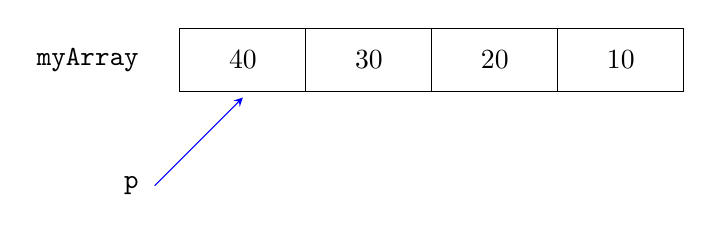
\begin{tikzpicture}[scale=0.8]
          \node[right] at (-0.5,0.5) [left] {\tt myArray};
          \draw (0,0) rectangle (8,1);
          \draw (2,0) -- (2,1);
          \draw (4,0) -- (4,1);
          \draw (6,0) -- (6,1);
          \node at (1,0.5) {$40$};
          \node at (3,0.5) {$30$};
          \node at (5,0.5) {$20$};
          \node at (7,0.5) {$10$};
          \node at (-0.5,-1.5) [left] {\tt p};
          \draw[blue,-stealth] (-0.4,-1.5) -- (1,-0.1);
        \end{tikzpicture}
      \end{minipage}
    \end{tabular}
  \end{center}
  \par\vskip 5pt
  
  {\it\large Refer to Model 1 above as your group develops consensus answers
    to the questions below.}
    \par\vskip 10pt
    
  \begin{enumerate}
    \itemsep 20pt
    
    \item The file {\tt activity05a.cpp} contains this code.
      Run it and record the output on the lines below.
      \par\vskip 15pt
      \begin{enumerate}
        \itemsep 15pt
        \begin{multicols}{2}
          \item {\tt Value of p: } \hfill \fillin[40][1.25in]
          \item {\tt Value of *p: } \hfill \fillin[a memory location][1.25in]
          \item {\tt Value of myArray: } \hfill \fillin[40,30,20,10][1.25in]
        \end{multicols}
      \end{enumerate}
      
    \item Run the code several times.  Describe how (if at all) the
      output changes each time you run the program.
      \begin{solution}[0.5in]
        Yes, the output from the first line changes each time it is run.
      \end{solution}

    \item A {\it pointer} is a variable that holds a memory address,
      rather than data.  The diagram on the right of the model
      depicts the pointer relationship in this code.
      \begin{enumerate}
        \item Based on the diagram, which variable is a pointer?
          \begin{solution}[0.5in]
          \end{solution}
        \item Now looking at the code, how is a pointer declared in C++?
          \begin{solution}[0.75in]
          \end{solution}
        \item How does this explain what you observed in question 2
          above?
          \begin{solution}[0.75in]
          \end{solution}
        \item Does a pointer have a data type like other variables? Explain.      
          \begin{solution}[0.75in]
          \end{solution}
      \end{enumerate}
      
    \item Now replace line 7 in the model with each of the following
      code snippets, one at a time.  Run the code and record its output.
      \par\vskip 10pt
      \begin{enumerate}
        \item \mintinline{cpp}|p++|
          \par\vskip 15pt          
          \begin{enumerate}
            \itemsep 15pt
            \begin{multicols}{2}
              \item {\tt Value of p: } \hfill \fillin[30][1.25in]
              \item {\tt Value of *p: } \hfill \fillin[a memory location][1.25in]
              \item {\tt Value of myArray: } \hfill \fillin[40,30,20,10][1.25in]
            \end{multicols}
          \end{enumerate}\par\vskip 10pt
        \item \mintinline{cpp}|(*p)++|
          \par\vskip 15pt
          \begin{enumerate}
            \itemsep 15pt
            \begin{multicols}{2}
              \item {\tt Value of p: } \hfill \fillin[41][1.25in]
              \item {\tt Value of *p: } \hfill \fillin[a memory location][1.25in]
              \item {\tt Value of myArray: } \hfill \fillin[41,30,20,10][1.25in]
            \end{multicols}
          \end{enumerate}\par\vskip 10pt
        \item \mintinline{cpp}|*(p+2) += 2;|
          \par\vskip 15pt
          \begin{enumerate}
            \itemsep 15pt
            \begin{multicols}{2}
              \item {\tt Value of p: } \hfill \fillin[40][1.25in]
              \item {\tt Value of *p: } \hfill \fillin[a memory location][1.25in]
              \item {\tt Value of myArray: } \hfill \fillin[40,30,22,10][1.25in]
            \end{multicols}
          \end{enumerate}
      \end{enumerate}
      
    \item Complete the diagram below to show the contents of
      {\tt myArray} and the pointer relationship between
      {\tt p} and {\tt myArray} after line 7 of the model 
      was changed as indicated above.
      \begin{enumerate}
        \begin{multicols}{2}
          \item \mintinline{cpp}|p++|\par\vskip 10pt
            \begin{minipage}{2.75in}
              \begin{tikzpicture}[scale=0.6]
                \node at (-0.5,0.5) [left] {\tt myArray};
                \draw (0,0) rectangle (8,1);
                \draw (2,0) -- (2,1);
                \draw (4,0) -- (4,1);
                \draw (6,0) -- (6,1);
                \node at (-0.5,-1.5) [left] {\tt p};
              \end{tikzpicture}
            \end{minipage}
          \item \mintinline{cpp}|(*p)++|\par\vskip 10pt
            \begin{minipage}{2.75in}
              \begin{tikzpicture}[scale=0.6]
                \node at (-0.5,0.5) [left] {\tt myArray};
                \draw (0,0) rectangle (8,1);
                \draw (2,0) -- (2,1);
                \draw (4,0) -- (4,1);
                \draw (6,0) -- (6,1);
                \node at (-0.5,-1.5) [left] {\tt p};
              \end{tikzpicture}
            \end{minipage}
        \end{multicols}
      \end{enumerate}
            
    \item Write a single line of code referencing only {\tt p} 
      that does the following when added \key\\[-2.5mm] on line 7.
      \par\vskip 15pt
      \begin{enumerate}[(a)]
        \itemsep 15pt
        \item Adds 5 to the first entry in {\tt myArray} (making it 45):
          \hfill\fillin[\mintinline{cpp}|*p += 5|][2in]
        \item Changes the second line of output to ``{\tt Value of *p: 10}'':
          \hfill\fillin[\mintinline{cpp}|p+=3|][2in]
        \item Adds 5 to the 2nd entry in {\tt myArray} (making it 35):
          \hfill\fillin[\mintinline{cpp}|*(p+2) += 5|][2in]          
      \end{enumerate}
      \par\vskip 10pt
      
    \item Finally, place the command \mintinline{cpp}|p -= 10;| on line 7
      of the model and run the code several times.
      \begin{enumerate}
        \item What happens to the output each time you run the program?
          \begin{solution}[0.75in]
          \end{solution}
        \item This example illustrates one of the {\it dangers} of
          using pointers.  In your own words, describe what that danger is.
          \begin{solution}[1.25in]
          \end{solution}
      \end{enumerate}


  {\bf\large Model 2: A Second Program with Pointers}\\[-10pt]
  \begin{center}
    \small
    \begin{minipage}{4.5in}
      \begin{minted}[
        frame=lines,
        framesep=2mm,
        bgcolor=gray!15,
        baselinestretch=1.2,
        linenos,
        firstnumber=4
      ]{cpp}
int main() {
  int numOne   = 1892;
  int numTwo   = 1973;
  int numThree = 2008;
  int* numArray[3] = { &numOne, &numTwo, &numThree };
  int* p;
  
  p = &numOne;
  cout << "Number: " << *p << endl;
  p = &numTwo;
  cout << "Number: " << *p << endl;
  p = &numThree;
  cout << "Number: " << *p << endl;
}
      \end{minted}
    \end{minipage}
  \end{center}
  
  {\it\large Refer to Model 2 above as your group develops consensus answers
    to the questions below.}
    \par\vskip 10pt
    
      \item Without running any code, predict what the output of this
        program will be.
        \begin{solution}[0.75in]
        \end{solution}
        
      \item The code for this model can be found in the file
        {\tt activity05b.cpp}.  Run this code and see if your
        predictions are correct.
        \begin{solution}[0.25in]
        \end{solution}        
        
      \item When dealing with pointers in C++, the symbol {\tt *} is
        called the {\it dereference operator}.  When it is placed in
        front of a pointer variable, it retrieves the data to which
        the pointer variable points.
        \par\vskip 10pt        
        \begin{enumerate}
          \item On which lines in the model above is the dereference
            operator used?
            \begin{solution}[1in]
            \end{solution}
            \vskip -30pt\null
          \item How would the output of this program change if the
            dereference operator were \key\\[-2.5mm] removed from those lines?
            \begin{solution}[1in]
            \end{solution}
          \item How does C++ tell the difference between a {\tt *}
            that is a dereference operator and a {\tt *} that indicates
            multiplication (i.e. \mintinline{cpp}|int x = 2 * y;|)?
            \begin{solution}[1in]
            \end{solution}
        \end{enumerate}

      \item The symbol {\tt \&} is called a {\it reference operator}.
        \par\vskip 10pt        
        \begin{enumerate}        
          \item On which lines in the model above is the reference
            operator used?
            \begin{solution}[1in]
            \end{solution}
\newpage            
          \item In your own words, describe what the reference
            operator does.
            \begin{solution}[1in]
              It returns the memory address (i.e. a reference) of the
              variable to which it is prepended.
            \end{solution}
          \item Is this usage of symbol {\tt \&} related to its usage
            to indicate ``pass-by-reference'' parameters in a function?
            Explain.
            \begin{solution}[1in]
            \end{solution}
          \item How would things changed if the reference operators 
            were removed from lines 11, 13, and 15 of the model?
            \begin{solution}[1in]
            \end{solution}
        \end{enumerate}
        
      \item Consider the array {\tt numArray} defined in this model.
        \par\vskip 10pt
        \begin{enumerate}
          \item What is the type of this array?
            \begin{solution}[0.75in]
            \end{solution}
          \item Describe the elements that are stored in this array.
            \begin{solution}[1in]
            \end{solution}
            \vskip -30pt\null
          \item Sketch a pointer diagram, similar to that seen in model 1,
            that depicts the values and\key\\[-2.5mm] pointer relationships of all
            five variables defined in model 2.
            \begin{solution}[1.6in]
            \end{solution}
        \end{enumerate}
        
      \item Suppose a new variable was defined as follows:
        \mintinline{cpp}|int** p2 = &numArray[1]|.
        \par\vskip 10pt
        \begin{enumerate}
          \item Describe both the type and purpose of the variable {\tt p2}.
            \begin{solution}[1in]
            \end{solution}
          \item What would be the output of each of the following commands?
            \par\vskip 15pt
            \begin{enumerate}
              \itemsep 15pt
              \item \mintinline{cpp}|cout << p2 << endl;|
                \hfill\fillin[a memory address][2.5in]
              \item \mintinline{cpp}|cout << *p2 << endl;|
                \hfill\fillin[a memory address][2.5in]
              \item \mintinline{cpp}|cout << **p2 << endl;|
                \hfill\fillin[a memory address][2.5in]
            \end{enumerate}
            \par\vskip 15pt
            
          \item Sketch a pointer diagram depicting the relationship 
            between the variable {\tt p2} and the rest of the
            variables in this model.
            \begin{solution}[1.25in]
            \end{solution}
        \end{enumerate}
        

  \end{enumerate}
       
\end{document}
